%! TEX root = ../main.tex

\section{Encuesta para evaluar la solución}
\label{sec:subjetiva}

Al final del período de prueba de la solución cada alumno que forma parte de la muestra
completa una encuesta con $31$ preguntas que se utilizan para validar las
consideraciones de diseño, las cuales fueron explicadas en el capítulo~\ref{chap:requerimientos}
y para medir sus apreciaciones sobre otros aspectos de la solución que serán
detallados más adelante en esta sección. 

Las preguntas están agrupadas en dos, el primer grupo cuenta con $27$ preguntas
cerradas, es decir de una sola respuesta en una lista de opciones, el segundo
grupo cuenta con $4$ preguntas abiertas, es decir los encuestados pueden dar
respuestas libres a las preguntas. 

De esta forma, se busca identificar las fortalezas y debilidades de la solución,
además de evaluar la solución en cuanto a factores de exploración,
representación, motivación, inmersión, retroalimentación y pedagogía, de acuerdo
a las apreciaciones de los miembros de la muestra.

\subsection{Muestra}

La encuesta es entregada a los $11$ alumnos de la población objetivo que acordaron
participar en la prueba y que fueron seleccionados como resultado de la 
\emph{Encuesta para determinar la muestra}, mientras completan la encuesta, un guía está presente
para responder cualquier duda.


\subsection{Variables}
\label{sec:variables}
%\observacion{Parece haber tanta referencia como para separar}

%A continuación se describen las variables que tienen por objetivo demostrar la
%validez de las consideraciones de diseño planteadas en este trabajo descritas en el
%capítulo~\ref{chap:requerimientos} y la medición de otros aspectos de la
%solución relacionados con los objetivos de este trabajo descritos en la
%sección~\ref{sec:objetivos_generales}. 

Las variables a medir son agrupadas en
factores, los cuales representan aquellos aspectos de la solución propuesta que
buscan ser evaluados.

Cabe resaltar que la medición de estas variables se realizan
exclusivamente de acuerdo a las valoraciones dadas por la muestra en cada una de
las preguntas que forman parte de la encuesta.

\subsubsection{Exploración}
\label{sec:sub_exploracion}
%\observacion{Creo que el nombre es confuso por que parece referirse al tema de
%interacción con el entorno}
%
%\observacion{Se podría simplificar el siguiente párrafo} 

Este factor se refiere a los aspectos de la solución que permiten al usuario 
explorar el entorno durante la partida. Para facilitar esta exploración se 
busca proveer  facilidad de uso, intuitividad y realismo en cuanto a las acciones y
situaciones que se presentan en la solución para que de esta manera, los
elementos que la componen no representen para el jugador un obstáculo que impida
su uso.

%Este factor esta \fixme{relacionado}{} con \fixme{la característica}{} que posee
%la solución en cuanto a la \fixme{oportunidad}{} que \fixme{brinda}{} al usuario
%para \fixme{explorar}{} cada uno de los elementos del entorno simulado
%(paciente, herramientas propias del procedimiento). En este sentido, se busca
%proveer facilidad de uso, intuitividad y realismo en cuanto a las acciones y
%situaciones que se presentan en la solución para que de esta manera, los
%elementos que la componen no representen para el jugador un obstáculo que impida
%su uso.
%\observacion{El factor que mide la eficiencia es acaso a explorar el entorno?}

Las variables que miden este aspecto son las siguientes:

\begin{description}



\item[Funciones realizadas por los elementos del juego:] se refiere a si las 
	simplificaciones realizadas en la solución en cuanto a las funciones de cada uno 
	de los elementos del juego facilitan su uso.

%se refiere a la
%    correctitud con la que una herramienta o elemento del juego representa las
%    funciones que el mismo puede realizar en la vida real, en este sentido, se
%    evalúa el realismo con el que es representado tal elemento.

\item[Aleatoriedad para afianzar conocimientos:] se refiere al beneficio que
    puede traer el hecho de que el estado del paciente en el juego sea aleatorio
    en cuanto a la posibilidad que esto brinda al jugador para poner a prueba
    sus conocimientos teóricos.

\item[Aleatoriedad para representar realismo:] se refiere al uso de estados
    aleatorios en el paciente para que de esta forma el procedimiento se asemeje
    más a una situación real e invite al usuario a explorar el entorno.

\item[Intuitividad:] se refiere a lo intuitivo que puede ser la
    utilización de los elementos del juego.

\end{description}

\subsubsection{Representación}
\label{sec:sub_representacion}

Este factor está relacionado con la calidad y suficiencia con la que se
representan los diferentes objetos que son simulados en la solución. La
representación abarca tanto funcionalidad como aspecto del objeto.

De esta manera, se busca permitir al usuario realizar con los objetos las
acciones que requiera para llevar a cabo el procedimiento que se le presente en
la solución, y además, representar estos elementos de la mejor manera posible.

Las variables que miden estos aspectos son las siguientes:

\begin{description}

\item [Respuestas del paciente:] se refiere a la suficiencia de las respuestas 
    motrices, oculares y verbales que realiza el paciente en la escena 
    correspondiente a la valoración de la escala de Glasgow.

\item[Distinción entre los estados del paciente:] se refiere a si los diferentes
    estados del paciente son distinguidos correctamente en el procedimiento de
    valoración de la escala de Glasgow ya que esto es importante para que el
    usuario pueda diagnosticar correctamente al paciente.

\item[Acciones con los elementos:] se refiere a si las diferentes acciones que
    pueden realizarse con los elementos o herramientas del juego en un
    determinado procedimiento de enfermería son suficientes para ese
    procedimiento, ya que, debido a las limitaciones de la tecnología estas
    acciones son limitadas.

\end{description}

\subsubsection{Motivación}
\label{sec:sub_motivacion}

Este factor está relacionado con la importancia de incluir en la solución
aquellas características lúdicas que son propias de un videojuego convencional. Se
busca conocer el valor de estas características en cuanto a la motivación que
puedan producir en los usuarios tanto para volver a utilizar la solución como
para superarse en cada partida.

Las variables que miden estos aspectos son las siguientes:

\begin{description}

\item[Motivación del puntaje:] se refiere a que tanto motiva al jugador que la
    solución le proporcione un puntaje total al final de cada partida para poder
    mejorar constantemente siendo este puntaje como una evaluación final de todo
    lo que realizó durante la partida.

\item[Importancia del puntaje:] se refiere a que tan importante es para un
    jugador que se le proporcione un puntaje total al final de cada partida para
    poder visualizar su rendimiento.

\item[Socialización de los puntajes:] se refiere a si el hecho de que las
    personas del mismo entorno compartan sus puntajes, experiencias y logros en
    las partidas a través de redes sociales pueda ser motivador.

\item[Medición del tiempo:] se refiere a que tanto motiva al
    jugador que la solución le proporcione el tiempo que duro su partida
    sirviendo este tiempo como una evaluación de su precisión a la hora de
    realizar el procedimiento que se le presente.

\end{description} 


\subsubsection{Inmersión}
\label{sec:sub_inmersion}

Este factor está relacionado con la percepción de formar
parte de la escena. Es decir, se trata de evaluar que tanto el usuario puede
sentir que realmente se encuentra dentro del juego para que de este modo el
pueda entrar en ambiente para realizar los procedimientos que se le presenten en
sus partidas de juego.

Las variables que miden este aspecto son las siguientes:

\begin{description}

\item[Escenografía para entrar en ambiente:] se refiere a la importancia de la
    escenografía de la partida para que el jugador entre en ambiente para
    realizar el procedimiento que se le presente.

\item[Juegos cortos:] se refiere a si el hecho de
    que los procedimientos presentados en las partidas sean cortos contribuye a
    repetir las partidas varias veces de seguido entrando en un estado de
    inmersión.

\item[Gráficos en tres dimensiones para entender el entorno:] se refiere a la
    importancia que tiene el uso de gráficos en tres dimensiones para que el
    usuario pueda entender mejor el entorno y las posibles acciones que puede
    realizar.

\item[Realismo a través de ordenes verbales:] se refiere a si el hecho de que la
    solución brinde la posibilidad de que aparezca un menú de ordenes verbales
    en el momento en que el jugador habla hace que la acción de dar ordenes
    verbales se asemeje más a la realidad.

\item[Sentido de pertenencia:] se refiere a si la simulación ayuda al
    jugador a sentirse parte del laboratorio, dando cierto realismo a la escena
    que se le presenta.

\end{description}

\subsubsection{Utilidad}
\label{sec:sub_utilidad}

Este factor está relacionado con el potencial de la solución como herramienta 
de apoyo al proceso de aprendizaje de los estudiantes de enfermería.

Las variables que miden este aspecto son las siguientes: 

\begin{description}
\item[Simulación para complementar el estudio en clase y laboratorio:] se
    refiere a que tanto potencial tienen las herramientas alternativas como la
    simulación para complementar a los métodos de aprendizaje tradicionales
    que son el estudio en clase y en el laboratorio.

\item[Simulación como proveedor de facilidades para el estudio:] se refiere a si las
    herramientas alternativas como la solución proveen más facilidades para
    poner en practica los conocimientos con respecto a los demás métodos de
    aprendizaje que son los libros, laboratorios y el campo de prácticas.

\item[Interacción con el paciente:] se refiere a si el hecho de que el jugador
    pueda interactuar con un paciente que responde a las acciones del jugador 
    implica una mejora con respecto a otros materiales utilizados en los 
    laboratorios de práctica.

\end{description}

%\observacion{Algunos parecen estar fuera de lugar (los que tienen ?)}

\subsubsection{Retroalimentación}
\label{sec:sub_retroalimentacion}

Este factor está relacionado con la importancia de ofrecer al jugador
información acerca de sus logros y errores de manera tal que el pueda estar
consciente de sus puntos fuertes y sus puntos débiles en los diversos
procedimientos que realice en la solución.

Las variables que miden este aspecto son las siguientes:

\begin{description}[style=unboxed]

\item[Detalles de los pasos realizados incorrectamente:] se refiere a 
    la importancia que tiene para el usuario que la solución no sólo le 
    diga los pasos que realizó de manera incorrecta sino también el por qué 
    de ello.

\item[Retroalimentación suficiente respecto a los pasos realizados:] se refiere 
    a si son suficientes las justificaciones breves acerca de las causas por las 
    cuales se realizó incorrectamente un paso.

\item[Representación iconográfica de conceptos y acciones en la \Gls{gui}:] 
    se refiere a la suficiencia de mostrar iconos en la interfaz de 
    la solución para representar el estado actual del jugador.

\end{description}

\subsubsection{Pedagogía}
\label{sec:sub_pedagogia}

Este factor está relacionado al beneficio que puede traer la
solución para apoyar el aprendizaje del jugador. De esta manera, se busca
obtener la validez real de este tipo de herramientas como aporte al aprendizaje,
proveyendo mas interacción al jugador.

Las variables que miden este aspecto son las siguientes:

\begin{description}

\item[Potencial para memorizar y comprender el procedimiento:] se refiere a
    que tanto ayuda la solución al usuario para entender los procedimientos que se
    le presentan y para no olvidar los pasos de cada uno de ellos.

\item[Retroalimentación limitada:] se refiere a que tan efectivo
    resulta no dar pistas al jugador en el momento de realizar un procedimiento
    para que pueda plasmar y medir sus conocimientos.

\item[Acciones a través de botones:] se refiere a que tan
    suficiente es representar determinadas acciones  con un botón debido a
    limitaciones en la tecnología.

\end{description}


\subsection{Métricas}

La métrica utilizada en las preguntas cerradas es la escala de Likert haciendo
uso de la \emph{Doble estandarización}, como se describe en la
sección~\ref{sec:likert}. Esto ayuda a determinar los puntos fuertes y débiles
de los aspectos evaluados.

Además se utilizan promedios hallados teniendo en cuenta las respuestas de los
usuarios en cada una de las preguntas cerradas para determinar el nivel de
aceptación promedio en cuanto a los temas abordados en las preguntas.

\subsubsection{Manejo de información faltante}
\label{sec:informacion_faltante}
%\observacion{No repetir tanto existe}

Debido a que hubieron preguntas no respondidas en una de las encuestas, se utilizaron 
métodos para tratar esa información faltante. En este tipo de situaciones existen tres 
posibles formas de categorizar el patrón de ocurrencia de la falta de 
respuestas\cite{leite2010performance, tsikriktsis2005review}:

\begin{description}
    \item[Información faltante completamente aleatoria:] cuando la información
        faltante es independiente de la variable medida y de otras variables.
    \item[Información faltante aleatoria:] cuando la información faltante depende
        de otras variables, pero no de la variable en sí. 
    \item[Información faltante no aleatoria:] cuando hay una relación entre la
        información faltante y el valor de la variable.
\end{description}

En esta caso el patrón corresponde al tipo \emph{Información faltante completamente aleatoria}. 
Existen a tres mecanismos~\cite{tsikriktsis2005review} principales para lidiar con información
faltante para este patrón: la eliminación, el sustitución y los  procedimientos basados en
modelo.~\cite{tsikriktsis2005review} recomienda utilizar un mecanismo de
reemplazo para escalas del tipo \textit{Likert}.

Las técnicas de sustitución se clasifican en tres grandes
grupos\cite{tsikriktsis2005review}:
\begin{enumerate*}[label=\itshape\alph*\upshape)]
\item basadas en el promedio,
\item basadas en regresión, e,
\item imputación \emph{hot deck}.
\end{enumerate*}

De estas técnicas se seleccionó \emph{la sustitución} basado en el 
promedio ya que las relaciones entre las variables son bajas y los datos
faltantes son menos del $10\%$. La sustitución basada por promedio se divide
nuevamente en tres grupos\cite{tsikriktsis2005review}; promedio
\begin{enumerate*}[label=\itshape\alph*\upshape.]
\item total,
\item del subgrupo, y,
\item por caso.
\end{enumerate*}

La sustitución por promedio total es elegida debido a que la relación entre la
variable que falta y las demás variables en los datos es relativamente baja, es
fácil de usar y retiene la muestra. 

%La sustitución por promedio total se realiza
%obteniendo el promedio de todas las respuestas de la pregunta cuya respuesta
%falte, la sustitución de subgrupo es similar, solo que se limita a aquellos
%sujetos del mismo subgrupo del sujeto que no respondió, y finalmente, la
%sustitución por caso, es el promedio de las respuestas válidas del sujeto.


\subsection{Resultados obtenidos}
\label{sec:res_subjetiva}

Los resultados obtenidos con la encuesta son separados en \emph{Preguntas cerradas} y 
\emph{Preguntas abiertas} para una mejor comprensión.

\subsubsection{Preguntas cerradas}
La tabla~\ref{tab:subjetiva_conformidad_exploracion} muestra 
las respuestas de los alumnos a las preguntas relacionadas al factor
exploración, son cuatro preguntas, las cuales fueron descritas
en~\ref{sec:sub_exploracion}. Según los datos, la simplificación de las funciones 
de los elementos es el punto con menor valoración, no obstante tiene una valoración 
promedio de \emph{Parcialmente de acuerdo}.
%\observacion{Revisar bien los tiempos}
%\observacion{En este punto uno ya se olvida de la escala}
%\observacion{Algo que resaltar de todas estas tablas?}

\begin{table}[H]
\centering
\begin{tabular}{@{} *{5}{r} @{}}
\toprule
& \multicolumn{4}{c}{Exploración} \\
\cmidrule(lr){2-5}
Alumno &
\parbox{2.5cm}{Facilidad de uso}  &
\parbox{3cm}{Funciones realizadas por los elementos del juego} &
\parbox{3cm}{Aleatoriedad para afianzar conocimientos} &
\parbox{2.5cm}{Aleatoriedad para representar realismo} \\
\midrule
1         & 2   & 6   & 5   & 6  \\
2         & 6   & 6   & 4   & 6  \\
3         & 3   & 3   & 5   & 5  \\
4         & 6   & 6   & 6   & 6  \\
5         & 6   & 6   & 2   & 5  \\
6         & 6   & 6   & 6   & 6  \\
7         & 7   & 7   & 7   & 7  \\
8         & 6   & 6   & 7   & 7  \\
9         & 5   & 7   & 7   & 7  \\
10        & 6   & 7   & 6   & 6  \\
11        & 7   & 6   & 7   & 6  \\
\midrule
\textbf{Promedio}  & \textbf{5}   & \textbf{6}   & \textbf{6}   & \textbf{6} \\
\bottomrule
\end{tabular}
\caption{Resultados de la \emph{Encuesta para evaluar la solución} relacionados al factor exploración}
\label{tab:subjetiva_conformidad_exploracion}
\end{table}

La tabla~\ref{tab:subjetiva_conformidad_representacion} agrupa las respuestas de
los alumnos según la calidad de representación, son cinco preguntas, las cuales
fueron descritas en~\ref{sec:sub_representacion}. Según los datos, los puntos débiles 
son las diferentes respuesta verbales que brinda el paciente virtual y la distinción 
entre los estados del paciente, ambos recibieron en promedio una valoración de 
\emph{Neutral}. El punto más fuerte tiene que ver con los movimientos motrices del 
paciente virtual, con una valoración promedio de \emph{De acuerdo}.

\begin{table}[H]
\centering
\begin{tabular}{@{} *{6}{r} @{}}
\toprule
& \multicolumn{5}{c}{Representación} \\
\cmidrule(lr){2-6}
& & \multicolumn{3}{c}{Respuestas del paciente} & \\
\cmidrule(lr){3-5}
Alumno &
\parbox{2.5cm}{Acciones con los elementos} &
\parbox{2.5cm}{Movimientos oculares del paciente} &
\parbox{2.5cm}{Reacción verbal del paciente} &
\parbox{2.5cm}{Movimientos motrices del paciente} &
\parbox{2.5cm}{Distinción entre los estados del paciente} \\
\midrule
1  & 6 & 6 & 2 & 5 & 2  \\
2  & 4 & 5 & 5 & 6 & 4  \\
3  & 5 & 3 & 3 & 3 & 3  \\
4  & 6 & 5 & 2 & 4 & 2  \\
5  & 2 & 2 & 6 & 6 & 6  \\
6  & 6 & 4 & 6 & 6 & 6  \\
7  & 7 & 6 & 5 & 7 & 5  \\
8  & 6 & 7 & 7 & 7 & 5  \\
9  & 5 & 6 & 2 & 7 & 6  \\
10 & 6 & 4 & 4 & 4 & 5  \\
11 & 6 & 4 & 6 & 6 & 5  \\
\midrule
\textbf{Promedio}  & \textbf{5} & \textbf{5} & \textbf{4} & \textbf{6} & \textbf{4} \\
\bottomrule
\end{tabular}
\caption{Resultados de la \emph{Encuesta para evaluar la solución} relacionados al factor
    representación}
\label{tab:subjetiva_conformidad_representacion}
\end{table}

La tabla~\ref{tab:subjetiva_conformidad_motivacion} muestra las respuestas de
los alumnos a las preguntas relacionadas al factor \textit{Motivación}, son
cinco preguntas, las cuales fueron descritas en~\ref{sec:sub_motivacion}. Según los datos, 
el punto débil es la socialización del rendimiento con una valoración promedio de 
\emph{Parcialmente de acuerdo}. 

\begin{table}[H]
\centering
\begin{tabular}{@{} *{5}{r} @{}}
\toprule
& \multicolumn{4}{c}{Motivación} \\
\cmidrule(lr){2-5}
Alumno &
\parbox{2.5cm}{Importancia del puntaje} &
\parbox{3cm}{Socialización de los puntajes} &
\parbox{3cm}{Medición del tiempo} &
\parbox{2.5cm}{Motivación del puntaje} \\
\midrule
1  & 6 & 4 & 4 & 7  \\
2  & 7 & 4 & 6 & 6  \\
3  & 6 & 6 & 5 & 6  \\
4  & 1 & 4 & 6 & 1  \\
5  & 2 & 2 & 7 & 7  \\
6  & 6 & 5 & 4 & 6  \\
7  & 7 & 7 & 6 & 7  \\
8  & 7 & 7 & 7 & 7  \\
9  & 7 & 7 & 7 & 7  \\
10 & 7 & 4 & 5 & 7  \\
11 & 5 & 4 & 5 & 6  \\
\midrule
\textbf{Promedio}  & \textbf{6}   & \textbf{5}   & \textbf{6}   & \textbf{6} \\
\bottomrule
\end{tabular}
\caption{Resultados de la \emph{Encuesta para evaluar la solución} relacionados al factor motivación}
\label{tab:subjetiva_conformidad_motivacion}
\end{table}

La tabla~\ref{tab:subjetiva_conformidad_inmersion} muestra las respuestas de
los alumnos a las preguntas relacionadas al factor \textit{Inmersión}, son
cinco preguntas, las cuales fueron descritas en~\ref{sec:sub_inmersion}. Según los datos, 
todos los puntos fueron valorados en promedio de la misma manera, \emph{De acuerdo}.

\begin{table}[H]
\centering
\begin{tabular}{@{} *{6}{r} @{}}
\toprule
& \multicolumn{5}{c}{Inmersión} \\
\cmidrule(lr){2-6}
Alumno &
\parbox{2.5cm}{Realismo a través de ordenes verbales}                 &
\parbox{2.5cm}{Escenografía para entrar en ambiente}                  &
\parbox{2.5cm}{Gráficos en tres dimensiones para entender el entorno} &
\parbox{2.5cm}{Sentido de pertenencia}                                &
\parbox{2.5cm}{Juegos cortos}           \\
\midrule
1  & 4 & 6 & 4 & 5 & 3  \\
2  & 6 & 6 & 6 & 6 & 6  \\
3  & 6 & 6 & 6 & 5 & 6  \\
4  & 4 & 6 & 7 & 5 & 6  \\
5  & 6 & 6 & 5 & 6 & 6  \\
6  & 6 & 6 & 6 & 4 & 4  \\
7  & 7 & 7 & 7 & 7 & 7  \\
8  & 6 & 7 & 7 & 7 & 7  \\
9  & 6 & 7 & 7 & 7 & 7  \\
10 & 6 & 3 & 4 & 6 & 6  \\
11 & 5 & 3 & 5 & 5 & 4  \\
\midrule
\textbf{Promedio}  & \textbf{6} & \textbf{6} & \textbf{6} & \textbf{6} & \textbf{6} \\
\bottomrule
\end{tabular}
\caption{Resultados de la \emph{Encuesta para evaluar la solución} relacionados al factor inmersión}
\label{tab:subjetiva_conformidad_inmersion}
\end{table}

La tabla~\ref{tab:subjetiva_conformidad_utilidad} agrupa las respuestas de los
alumnos según la utilidad de la solución, son tres preguntas, las cuales fueron
descritas en~\ref{sec:sub_utilidad}. Según los datos, el punto débil se da en cuanto 
a la utilidad de utilizar al paciente virtual en comparación con un maniquí, con una 
valoración promedio de \emph{Parcialmente de acuerdo}.


\begin{table}[H]
\centering
\begin{tabular}{@{} *{6}{r} @{}}
\toprule
& \multicolumn{3}{c}{Utilidad} \\
\cmidrule(lr){2-4}
Alumno &
\parbox{4cm}{Interacción con el paciente} &
\parbox{4cm}{Provee facilidades para el estudio} &
\parbox{4cm}{Complementa el estudio en clase y laboratorio} \\
\midrule
1  & 7 & 5 & 7  \\
2  & 6 & 6 & 6  \\
3  & 6 & 6 & 6  \\
4  & 2 & 6 & 6  \\
5  & 2 & 6 & 6  \\
6  & 6 & 6 & 6  \\
7  & 7 & 6 & 7  \\
8  & 5 & 6 & 7  \\
9  & 7 & 7 & 7  \\
10 & 1 & 7 & 7  \\
11 & 6 & 4 & 5  \\
\midrule
\textbf{Promedio}  & \textbf{5} & \textbf{6} & \textbf{6} \\
\bottomrule
\end{tabular}
\caption{Resultados de la \emph{Encuesta para evaluar la solución} relacionados al factor utilidad}
\label{tab:subjetiva_conformidad_utilidad}
\end{table}

La tabla~\ref{tab:subjetiva_conformidad_retroalimentacion} agrupa las respuestas
de los alumnos según la calidad de retroalimentación, son tres preguntas, las
cuales fueron descritas en~\ref{sec:sub_retroalimentacion}. Según los datos, los puntos 
débiles son la representación del estado de los objetos de la simulación a través de imágenes y 
el nivel de detalle brindado al usuario acerca de las razones por las que no realizó 
correctamente un paso, ambos poseen una valoración promedio de \emph{Parcialmente de acuerdo}.

\begin{table}[H]
\centering
\begin{tabular}{@{} *{4}{r} @{}}
\toprule
& \multicolumn{3}{c}{Retroalimentación} \\
\cmidrule(lr){2-4}
Alumno &
\parbox{4cm}{Representación iconográfica de conceptos y acciones en la \Gls{gui}}  &
\parbox{4cm}{Retroalimentación suficiente respecto a los pasos realizados} &
\parbox{4cm}{Detalles de los pasos realizados incorrectamente} \\
\midrule
1  & 3 & 2 & 7  \\
2  & 5 & 4 & 6  \\
3  & 3 & 6 & 6  \\
4  & 6 & 6 & 6  \\
5  & 6 & 1 & 6  \\
6  & 2 & 6 & 6  \\
7  & 6 & 7 & 7  \\
8  & 6 & 6 & 7  \\
9  & 6 & 6 & 7  \\
10 & 5 & 4 & 6  \\
11 & 4 & 5 & 6  \\
\midrule
\textbf{Promedio}  & \textbf{5} & \textbf{5} & \textbf{6} \\
\bottomrule
\end{tabular}
\caption{Resultados de la \emph{Encuesta para evaluar la solución} relacionados al factor
    retroalimentación}
\label{tab:subjetiva_conformidad_retroalimentacion}
\end{table}

La tabla~\ref{tab:subjetiva_conformidad_pedagogia} agrupa las respuestas de los
alumnos según el factor pedagógico, son tres preguntas, las cuales fueron
descritas en~\ref{sec:sub_pedagogia}.  Según los datos, 
todos los puntos fueron valorados en promedio de la misma manera, \emph{Pacialmente de acuerdo}.

%\observacion{Habrá que replantear algunos nombres (falta de pistas como)}
\begin{table}[H]
\centering
\begin{tabular}{@{} *{4}{r} @{}}
\toprule
& \multicolumn{3}{c}{Pedagogía} \\
\cmidrule(lr){2-4}
Alumno &
\parbox{4cm}{Acciones a través de botones} &
\parbox{4cm}{Retroalimentación limitada} &
\parbox{4cm}{Potencial para comprender el procedimiento} \\
\midrule
1  & 6 & 6 & 6  \\
2  & 6 & 6 & 7  \\
3  & 4 & 6 & 6  \\
4  & 6 & 7 & 6  \\
5  & 7 & 5 & 6  \\
6  & 4 & 4 & 6  \\
7  & 7 & 6 & 7  \\
8  & 6 & 7 & 7  \\
9  & 7 & 7 & 7  \\
10 & 6 & 7 & 7  \\
11 & 5 & 6 & 5  \\
\midrule
\textbf{Promedio}  & \textbf{6} & \textbf{6} & \textbf{6} \\
\bottomrule
\end{tabular}
\caption{Resultados de la \emph{Encuesta para evaluar la solución} relacionados al factor pedagogía}
\label{tab:subjetiva_conformidad_pedagogia}
\end{table}

%\subsubsection{Agrupamiento de datos}

Los resultados se resumen en la tabla~\ref{tab:subjetiva_conformidad_resumen},
donde se muestra el número de alumno para identificar a un alumno y el promedio de sus
respuestas en la encuesta por factor estudiado. Se puede observar que el promedio total por 
cada factor indica que los de menor valoración son la representación y la retroalimentación 
con una valoración promedio de \emph{Parcialmente de acuerdo}.


Como se explica en la sección~\ref{sec:likert}, estos resultados están sujetos a
tendencias, para ello se aplica el método de doble
estandarización\cite{Pagolu2011}.

%, se muestra el promedio de las mismas.

%\observacion{Retroalimentación esta marcado con un circulo}

\begin{table}[H]
\centering
\begin{tabular}{llllllllr}
\toprule
\textbf{\shortstack{Número de \\alumno}}         &
\begin{sideways}\textbf{Motivación}                    \end{sideways}        &
\begin{sideways}\textbf{Exploración}                     \end{sideways}        &
\begin{sideways}\textbf{Inmersión}                       \end{sideways}        &
\begin{sideways}\textbf{Pedagogía}                       \end{sideways}        &
\begin{sideways}\textbf{Representación}                  \end{sideways}        &
\begin{sideways}\textbf{Retroalimentación}               \end{sideways}        &
\begin{sideways}\textbf{Utilidad}                        \end{sideways}        &
\textbf{\shortstack{Promedio\\de respuestas}}\\
\midrule
1              & 5 & 5 & 4 & 6 & 4 & 4 & 6 & 5 \\
2              & 6 & 6 & 6 & 6 & 5 & 5 & 6 & 6 \\
3              & 4 & 6 & 6 & 5 & 3 & 5 & 6 & 5 \\
4              & 6 & 3 & 6 & 6 & 4 & 6 & 5 & 5 \\
5              & 5 & 5 & 6 & 6 & 4 & 4 & 5 & 5 \\
6              & 6 & 5 & 5 & 5 & 6 & 5 & 6 & 5 \\
7              & 7 & 7 & 7 & 7 & 6 & 7 & 7 & 7 \\
8              & 7 & 7 & 7 & 7 & 6 & 6 & 6 & 7 \\
9              & 7 & 7 & 7 & 7 & 5 & 6 & 7 & 6 \\
10             & 6 & 6 & 5 & 7 & 5 & 5 & 5 & 5 \\
11             & 7 & 5 & 4 & 5 & 5 & 5 & 5 & 5 \\
\midrule
Promedio Total & 6 & 6 & 6 & 6 & 5 & 5 & 6 & 6 \\
\bottomrule
\end{tabular}
\caption{Resultados de la \emph{Encuesta para evaluar la solución}}
\label{tab:subjetiva_conformidad_resumen}
\end{table}

%Se observa que el puntaje más bajo en el promedio final es 5 que significa
%\textit{Parcialmente de acuerdo}, y el más alto es 7, que significa
%\textit{Totalmente de acuerdo}, se observa además el puntaje 6, que significa
%\textit{De acuerdo}. 

Con el resultado final de la estandarización diferenciamos cuáles son los puntos
fuertes y cuáles los puntos débiles de la solución propuesta con respecto a las
respuestas dadas por los usuarios. Estos valores son relativos a las respuestas
originales dadas en la encuesta, los resultados se muestran en la
tabla~\ref{tab:subjetiva_conformidad_corregida}. Los datos demuestran que, el punto 
más fuerte es la utilidad seguida de la exploración, el punto más débil es la representación 
seguida de la retroalimentación. De esta forma se puede valorar mejor cada uno de los factores 
a diferencia de los datos mostrados en~\ref{tab:subjetiva_conformidad_resumen}.

\begin{table}[H]
\centering
\begin{tabular}{lrrrrrrrr}
\toprule
\textbf{\shortstack{Número de \\alumno}}                                &
\begin{sideways}\textbf{Motivación}                    \end{sideways} &
\begin{sideways}\textbf{Exploración}                     \end{sideways} &
\begin{sideways}\textbf{Inmersión}                       \end{sideways} &
\begin{sideways}\textbf{Pedagogía}                       \end{sideways} &
\begin{sideways}\textbf{Representación}                  \end{sideways} &
\begin{sideways}\textbf{Retroalimentación}               \end{sideways} &
\begin{sideways}\textbf{Utilidad}                        \end{sideways} &
\textbf{\shortstack{Promedio\\de respuestas}}\\
\midrule
1              & 0.45 & 0.55 & 0.20 & 0.63 & 0.44 & 0.41 & 0.82 & 0.47 \\
2              & 0.33 & 0.53 & 0.49 & 0.61 & 0.27 & 0.13 & 0.52 & 0.41 \\
3              & 0.17 & 0.86 & 0.87 & 0.67 & 0.13 & 0.67 & 1.00 & 0.60 \\
4              & 0.75 & 0.31 & 0.63 & 0.81 & 0.47 & 0.78 & 0.54 & 0.59 \\
5              & 0.46 & 0.58 & 0.69 & 0.67 & 0.57 & 0.50 & 0.54 & 0.58 \\
6              & 1.00 & 0.73 & 0.68 & 0.42 & 0.90 & 0.67 & 1.00 & 0.78 \\
7              & 1.00 & 0.79 & 1.00 & 0.67 & 0.50 & 0.87 & 0.78 & 0.80 \\
8              & 0.75 & 1.00 & 0.83 & 0.75 & 0.70 & 0.70 & 0.44 & 0.75 \\
9              & 0.90 & 1.00 & 0.93 & 1.00 & 0.64 & 0.92 & 1.00 & 0.90 \\
10             & 0.79 & 0.74 & 0.54 & 0.92 & 0.60 & 0.60 & 0.67 & 0.68 \\
11             & 0.75 & 0.42 & 0.08 & 0.25 & 0.60 & 0.35 & 0.25 & 0.39 \\
\midrule
\textbf{Promedio Total} & 0.67 & 0.68 & 0.63 & 0.67 & 0.53 & 0.60 & 0.69 & 0.63 \\
\bottomrule
\end{tabular}
\caption{Resultados de la \emph{Encuesta para evaluar la solución} con doble estandarización}
\label{tab:subjetiva_conformidad_corregida}
\end{table}

%Es importante notar que los datos de la
%tabla~\ref{tab:subjetiva_conformidad_corregida} son relativas a los datos de la
%tabla~\ref{tab:subjetiva_conformidad_resumen}, es decir, que la representación
%es el punto más débil, aún así, se ve que
%en~\ref{tab:subjetiva_conformidad_resumen} que el valor es $5$ de $7$, lo que
%indica que es un punto aceptable, y entre los factores analizados es el que
%menos aprobación obtuvo.

En la tabla~\ref{tab:resultado_resumen_aspectos_aceptacion} se puede observar el 
resumen de las tablas~\ref{tab:subjetiva_conformidad_resumen} y~\ref{tab:subjetiva_conformidad_corregida}.

%
%Adicionalmente, se puede \emph{Evaluar los puntos fuertes y débiles de la
%    solución}, utilizando los datos con doble estandarización de la
%tabla~\ref{tab:subjetiva_conformidad_corregida}, se crea la
%tabla~\ref{tab:resultado_resumen_aspectos_aceptacion}, donde se observa la
%apreciación de los usuarios por cada aspecto estudiado.

\begin{table}[H]
\centering
\begin{tabular}{lcr}
\toprule
Factores        & Promedio Subjetiva      & Promedio estandarizado \\
\midrule
Motivación        & De acuerdo              & $0.67$  \\
Exploración       & De acuerdo              & $0.68$  \\
Inmersión         & De acuerdo              & $0.63$  \\
Pedagogía         & De acuerdo              & $0.67$  \\
Representación    & Parcialmente de acuerdo & $0.53$  \\
Retroalimentación & Parcialmente de acuerdo & $0.60$  \\
Utilidad          & De acuerdo              & $0.69$  \\
\bottomrule
\end{tabular}
\caption{Aceptación por aspecto de la solución}
\label{tab:resultado_resumen_aspectos_aceptacion}
\end{table}

Para  obtener una mejor visión de las fortalezas y debilidades de la solución
propuesta, se presenta el gráfico de \emph{kiviat}~\ref{fig:subjetiva_kiviat}.

%\observacion{Pulir la manera en la que hacen referencia a este tópico, aclarando
%que son percepciones desde el punto de vista del usuario}
\begin{figure}[H]
\centering
\begin{tikzpicture}[label distance=.15cm]
\tkzKiviatDiagram[scale=1,%
                    lattice=9,
                    %step=10,
                    ]
                {Motivación,
                 Facilidad de Exploración,
                 Sensación de Inmersión,
                 Pedagogía,
                 Representación,
                 Retroalimentación,
                 Utilidad}
\tkzKiviatLine[thick,
                color=blue!25!white,
                mark=ball,
                ball color=blue,
                mark size=5pt,
                opacity=.2, 
                fill=blue!20](6.7,6.8,6.3,6.7,5.3,6.0,6.9)
\tkzKiviatGrad[prefix={$0,$},unity=1](1) 
\end{tikzpicture}
\label{fig:subjetiva_kiviat}
\caption{Gráfico de Kiviat de los factores evaluados}
\end{figure}

%Se observa que las principales debilidades de la solución son la representación
%y la retroalimentación, y las fortalezas la utilidad, pedagogía, exploración, y
%la motivación.

Por último, con las informaciones obtenidas de las respuestas de los usuarios a la encuesta, es posible 
\emph{Validar las consideraciones de diseño asumidas
    durante el desarrollo de la solución}, lo cual es uno de los objetivos de
este capítulo. En la tabla~\ref{tab:resultado_resumen_hipotesis} se observa la
opinión de los alumnos con respecto a las consideraciones de diseño asumidas
en~\ref{sec:hipotesis}, todas las consideraciones fueron aceptadas.

%\begin{table}[!hbt]
%\centering
%\begin{tabular}{lcr}
%\toprule
%Hipótesis                        & Promedio encuesta      & Promedio estandarizado \\
%\midrule
%Comandos de voz con interfaz     & De acuerdo              & $0,55$ \\
%Extracción uniforme de elementos & Parcialmente de acuerdo & $0,65$ \\
%Acciones de bioseguridad         & De acuerdo              & $0,58$ \\
%Representación iconográfica      & Parcialmente de acuerdo & $0,53$ \\
%Factores motivadores             & De acuerdo              & $0,65$ \\
%Falta de pistas                  & De acuerdo              & $0,61$ \\
%\bottomrule
%\end{tabular}
%\caption{Hipótesis con su aceptación}\label{tab:resultado_resumen_hipotesis}
%\end{table}

\begin{table}[H]
\centering
\begin{tabular}{lcr}
\toprule
& \multicolumn{2}{c}{Promedio} \\
%\cmidrule(c){2-3} 
\cmidrule(lr){2-3}
Consideraciones de diseño          & Encuesta                & Estandarizado \\
\midrule
C1. Interacción a través de la voz & De acuerdo              & $0,55$ \\
C2. Extracción de elementos        & Parcialmente de acuerdo & $0,65$ \\
C3. Bioseguridad                   & De acuerdo              & $0,58$ \\
C4. Representación Iconográfica    & Parcialmente de acuerdo & $0,53$ \\
C5. Motivación                     & De acuerdo              & $0,65$ \\
C6. Retroalimentación limitada     & De acuerdo              & $0,61$ \\
C7. Movilidad                      & De acuerdo              & $0,66$ \\
\bottomrule
\end{tabular}
\caption{Aceptación por consideración de diseño}
\label{tab:resultado_resumen_hipotesis}
\end{table}

\subsection{Preguntas abiertas}
\label{sec:res_subjetiva_abiertas}

La parte final de la encuesta que respondieron los alumnos cuenta con preguntas abiertas, 
donde los alumnos expresaron sus
opiniones sobre los aspectos que rodean al uso de este tipo de soluciones al
aprendizaje de enfermería.


\begin{itemize}
    \item El $100\%$ de los alumnos mencionó que este tipo de soluciones son
        beneficiosas para el aprendizaje de procedimientos de enfermería.
    \item El $64\%$ de los alumnos mencionó que la principal dificultad para
        utilizar la solución es el factor tiempo.
    \item El $45\%$ de los alumnos mencionó que la solución es completa,
        mientras que el $18\%$ sugirió más elementos e interacción con el
        paciente.
\end{itemize}


Con esta información se puede \emph{determinar el nivel de aceptación de la
    solución}, se observa que el $100\%$ de los alumnos cree que es beneficioso
contar con este tipo de soluciones.
